\begin{figure}[ht]
    \centering
    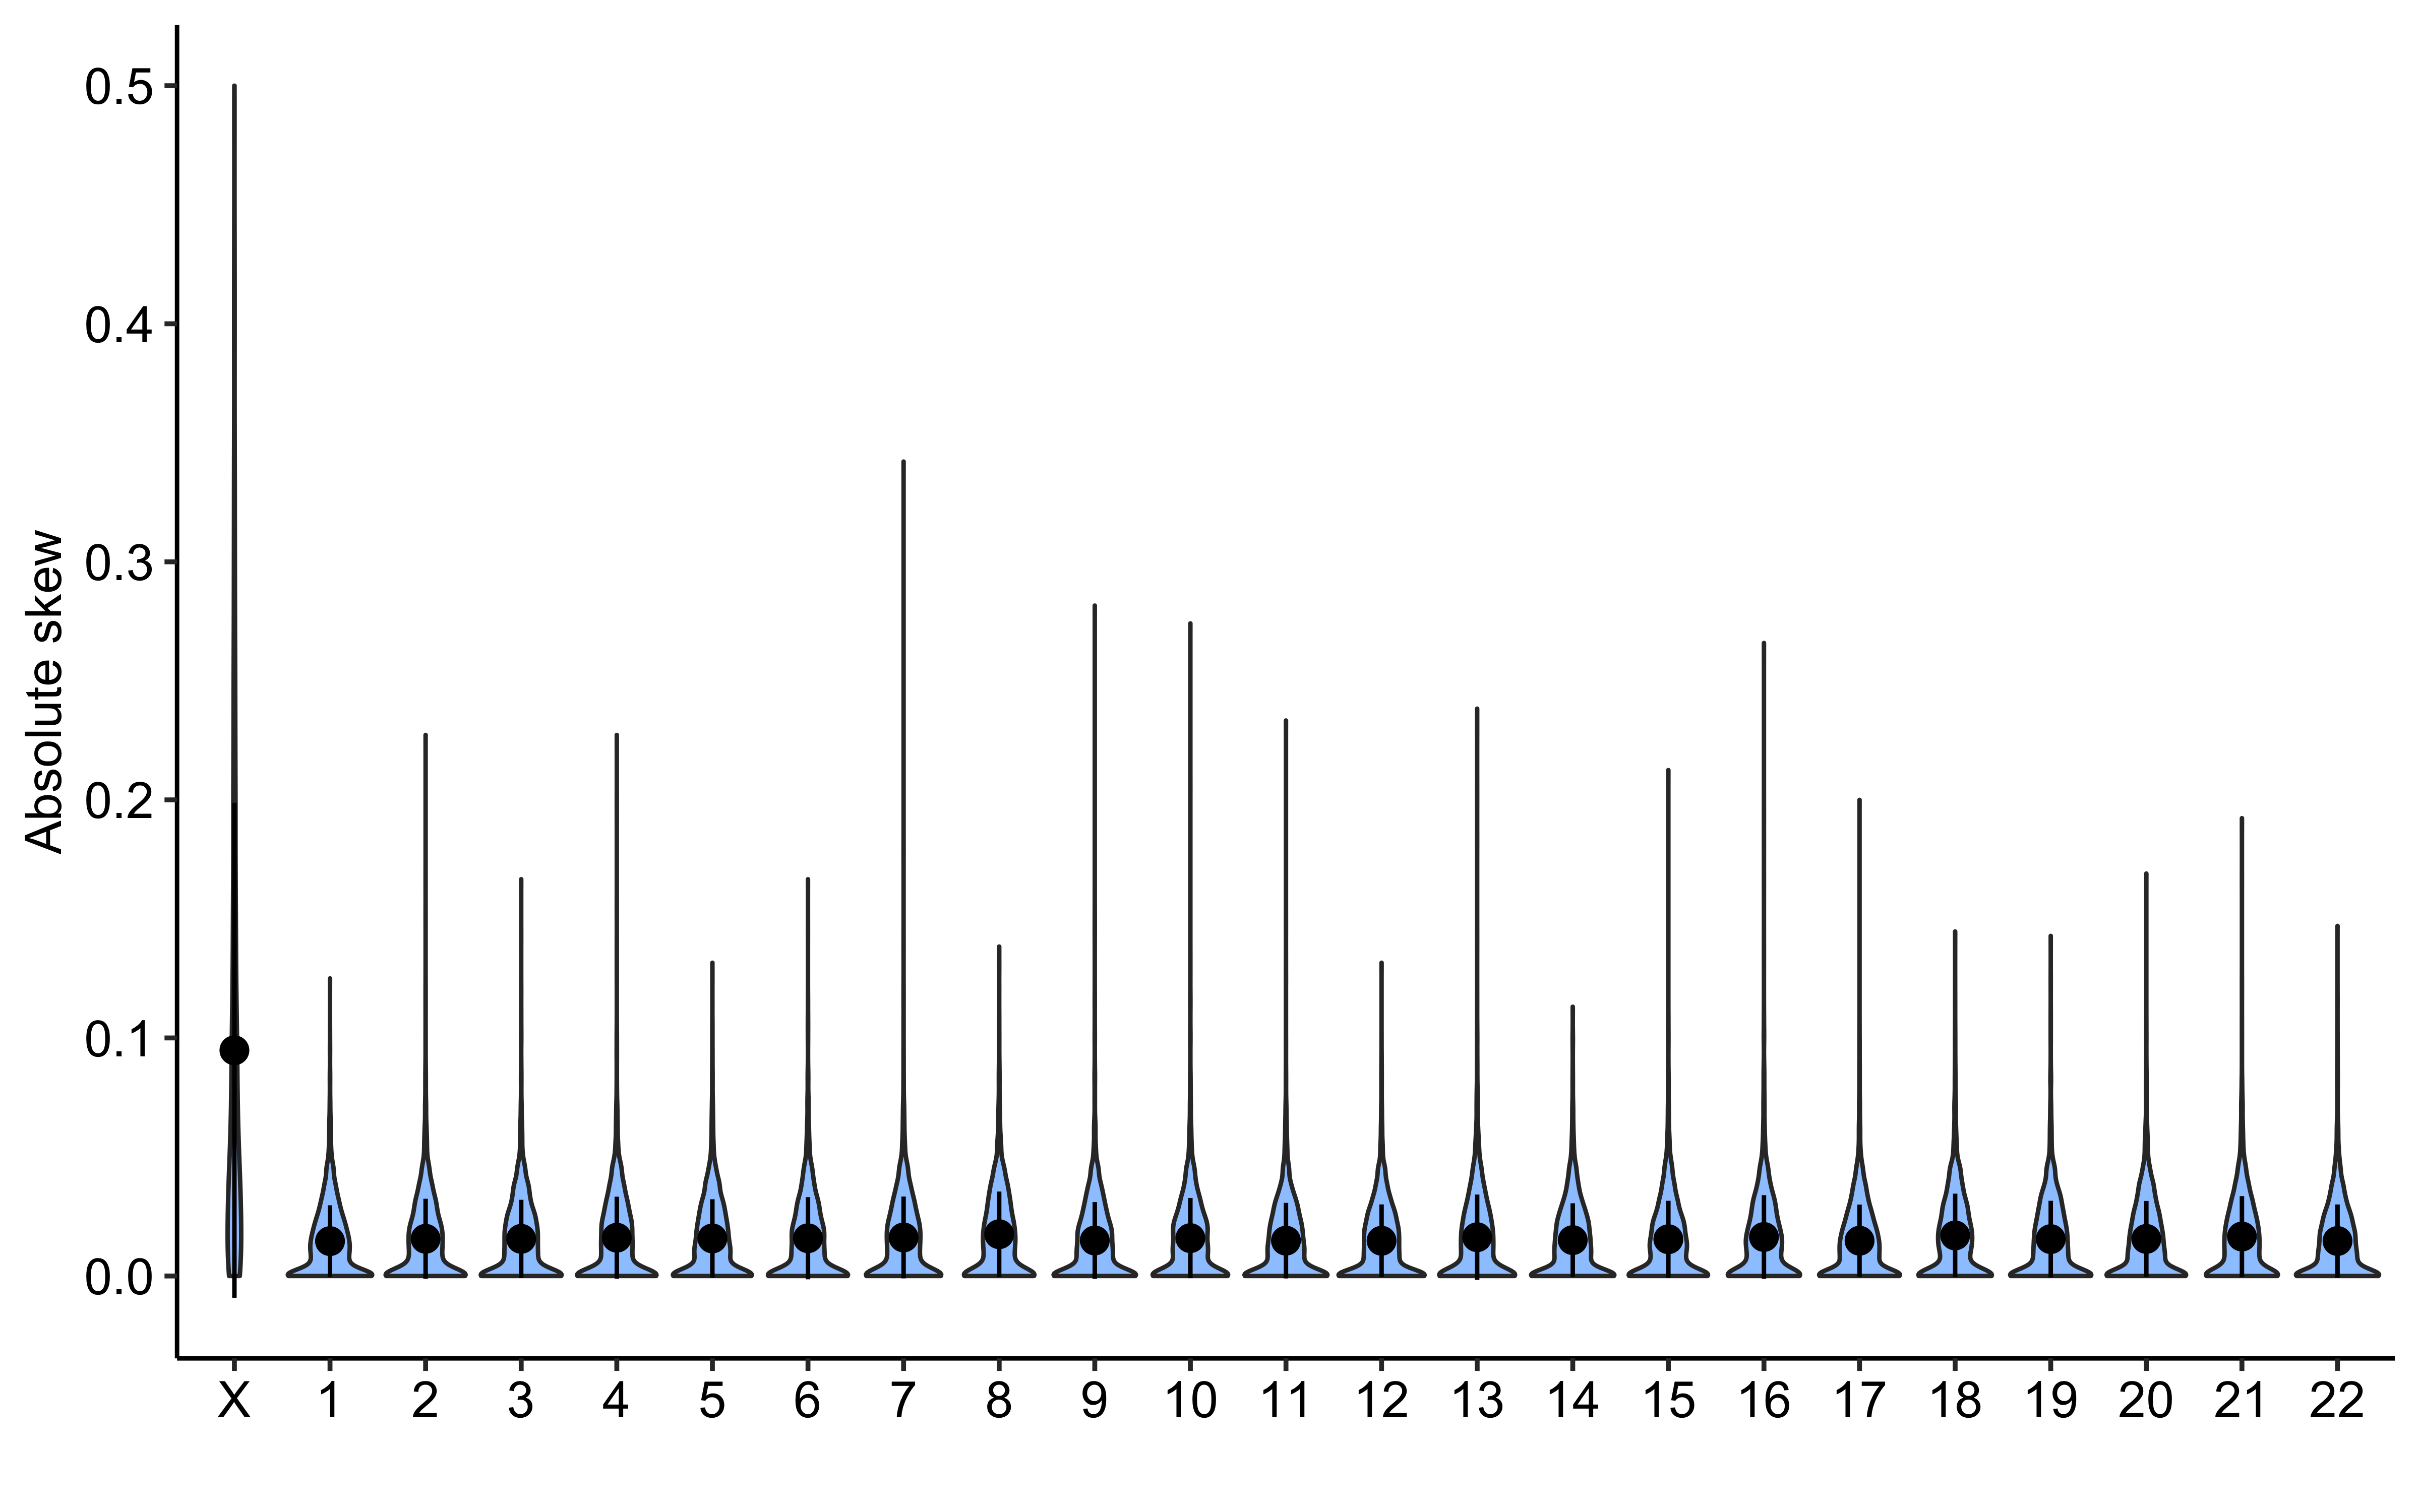
\includegraphics[width=0.75\textwidth]{chapter4/Figures/Supplementary_Figure_3.png}
    \caption{
        Estimated absolute skew in expression at heterozygous sites on the X chromosome and non-acrocentric autosomes. On the X chromosome, this value is used as the estimate of inactivation skewing since heterozygous sites are within fully inactivated genes. On the autosomes, an equal number of heterozygous sites used on the X chromosome for each sample were randomly selected from the q-arm to estimate the median skew in expression. Dots indicate mean of absolute skew with vertical lines indicating one standard deviation.
    }
    \label{fig:supp_fig4.3}
\end{figure}